\documentclass[man,noapacite]{apa} 

\usepackage{url}
\usepackage{apacite2}
\usepackage{amssymb}
\usepackage{graphicx}
\usepackage{xcolor}
\usepackage{listings}

% from http://tex.stackexchange.com/questions/110722/trying-to-include-r-code-with-listings-package
\lstset{ %
  language=R,                     % the language of the code
  basicstyle=\footnotesize\ttfamily,       % the size of the fonts that are used for the code
  numbers=none,                   % where to put the line-numbers
  numberstyle=\tiny\color{gray},  % the style that is used for the line-numbers
  stepnumber=1,                   % the step between two line-numbers. If it's 1, each line
                                  % will be numbered
  numbersep=5pt,                  % how far the line-numbers are from the code
  backgroundcolor=\color{white},  % choose the background color. You must add \usepackage{color}
  showspaces=false,               % show spaces adding particular underscores
  showstringspaces=false,         % underline spaces within strings
  showtabs=false,                 % show tabs within strings adding particular underscores
  % frame=single,                   % adds a frame around the code
  rulecolor=\color{black},        % if not set, the frame-color may be changed on line-breaks within not-black text (e.g. commens (green here))
  tabsize=2,                      % sets default tabsize to 2 spaces
  captionpos=b,                   % sets the caption-position to bottom
  breaklines=true,                % sets automatic line breaking
  breakatwhitespace=false,        % sets if automatic breaks should only happen at whitespace
  title=\lstname,                 % show the filename of files included with \lstinputlisting;
                                  % also try caption instead of title
  keywordstyle=\color{blue},      % keyword style
  commentstyle=\color{green!60!black},   % comment style
  stringstyle=\color{green!60!black},      % string literal style
  escapeinside={\%*}{*)},         % if you want to add a comment within your code
  morekeywords={*,...},           % if you want to add more keywords to the set
  belowskip=-2 \baselineskip,
  otherkeywords={%  
    filter, group_by, select, summarise, left, join, mutate, summarise_each
    }, 
    deletekeywords={data, get, median, na}
} 

\newcommand{\comment}[1]{\marginpar[]{\small \textcolor{blue}{#1}}}


%%%%%%%%%%%%%%%%%%%%%% MAIN TEXT STARTS HERE %%%%%%%%%%%%%%%%%%%%%%

\title{Wordbank: An Open Repository for Developmental Vocabulary Data} 

\author{~}
\affiliation{~}
% \author{Michael C. Frank, Mika Braginsky, Daniel Yurovsky, \\ \& Virginia A. Marchman} 
% \affiliation{Department of Psychology, Stanford University}

\abstract{The MacArthur-Bates Communicative Development Inventories (CDIs) are a widely-used family of parent-report instruments for easy and inexpensive data-gathering about early language acquisition. CDI data have been used to explore a variety of theoretically-important topics, but with few exceptions, researchers have had to rely on data collected in their own lab: there is no resource that offers researchers the opportunity to share and access raw CDI data. We describe Wordbank, a structured database of vocabulary measures from CDI forms combined with a browsable web interface. Wordbank archives CDI data across languages and labs, providing a resource for researchers interested in early language as well as a platform for novel analyses. The site allows interactive exploration of patterns of vocabulary growth at the level of both individuals and particular words. We also introduce wordbankr, a software package for connecting to the platform directly.}

\shorttitle{Wordbank: A Repository For Vocabulary Data} 
\rightheader{WORDBANK: A REPOSITORY FOR VOCAB DATA}

\acknowledgements{~}
% \acknowledgements{This work supported by a John Merck Scholars award and NSF BCS-1528526. Thanks to Ranjay Krishna for contributions to the initial development of the site, to Rune N\o rgaard J\o rgensen for helping port data from CLEX, to all of the contributors listed at \url{wordbank.stanford.edu/contributors} for generously sharing their data, and to the Advisory Board of the MacArthur-Bates Communicative Development Inventories, especially Philip Dale and Larry Fenson, for their support. 

% Please address correspondence to Michael C. Frank, Department of Psychology, Jordan Hall (Bldg. 420), 450 Serra Mall, Stanford, CA 94305. Phone: (650) 724-4003. E-mail: \url{mcfrank@stanford.edu}.}

\begin{document}

\maketitle

\section{Introduction}

% In addition, since vocabulary growth lays the groundwork for future academic achievement \cite{hart1995,marchman2008}, a better scientific understanding of factors affecting vocabulary development holds the promise of societal benefits.

Learning language is one of the most impressive and intriguing human accomplishments: Understanding the processes by which vocabulary grows provides a window into mechanisms of linguistic and cognitive development more generally \cite{bloom2002}. The MacArthur-Bates Communicative Development Inventories \cite<CDIs;>{fenson1994,fenson2007} are a widely-used family of parent-report instruments for easy and inexpensive data-gathering about early language acquisition. CDI data have been used to explore many theoretically-rich topics, including variation in early word production \cite{fenson1994}, vocabulary composition \cite{bates1994}, and the growth of lexical networks \cite{hills2009}. With few exceptions, however, researchers have had to rely on data collected in their own lab. While CDI norms are available \cite{fenson2007,jorgensen2010}, no public resource offers researchers the opportunity to share and access raw, cross-linguistic data at the scale necessary to address questions about demographic variation, vocabulary composition, relations with grammatical development, and other important issues.

To remedy this issue, we introduce Wordbank (\url{wordbank.stanford.edu}), a structured database of developmental vocabulary data. Building on previous tools like CLEX \cite{jorgensen2010}, Wordbank archives raw CDI data across languages and labs, providing a large-scale database of information about children's vocabulary knowledge. The site hosts an interactive and expandable set of in-depth analyses that can be explored by interested researchers, students, and members of the public. Wordbank lowers the cost of new, exploratory analyses by facilitating the productive reuse of data.

The current paper presents the Wordbank site in detail. We begin by discussing the motivations for constructing such a site. The bulk of the paper then describes the Wordbank site, including its database architecture, its web-based front-end, and its extensibility. We end by presenting \texttt{wordbankr}, a package for the \texttt{R} statistical programming language that allows research users to access the database directly, showing as a case study an analysis of gender differences in productive vocabulary across languages. 

\section{Motivation and Background} 

The nature and course of early word learning is an important window into children's growing understanding of the world. Early words cross-cut a variety of linguistic categories, but generally consist of names for caregivers (e.g., mama), common objects (e.g., bottle, shoe), social expressions (e.g., bye-bye), and actions or routines (e.g., peekaboo, throw) \cite{nelson1973,tardif2008}. New words enter children's expressive vocabularies slowly at first but this process accelerates over the second year such that children reach an average of 300 words by 24 months and more than 60,000 by the time they graduate from high school \cite{fenson2007}. At the same time, there are significant individual differences in language acquisition. For example, according to detailed observational studies, although some 18-month-olds already produce 50--75 words, others produce no words at all, and will not do so until they are 22 months or older \cite<e.g.,>{brown1973,bloom2002,clark2003}. How can such differences be measured accurately and efficiently? And can we promote early detection of differences in vocabulary growth that will be clinically significant later in development? 

\subsection{Measuring early vocabulary}

Traditional studies of language development typically apply a combination of observational assessment and structured tests, frequently relying on short samples of interactions and small samples of children. Discerning both the universal features and natural variation in early lexical development has been greatly facilitated by the development of parent report instruments like the MacArthur-Bates CDI \cite{fenson1994,fenson2007} and the Language Development Survey \cite{rescorla1989}. The CDIs were developed across a period of more than 40 years. Originally designed for use in a research study \cite{bates1976}, the instruments have evolved from a structured interview to the current paper-and-pencil format and are now increasingly administered online (e.g., \citeNP{kristoffersen2013} for Norwegian or \url{http://laboratorium.detskarec.sk} for Slovak). While other assessment tools exist for slightly older children, to our knowledge, no other measure allows cost-effective global language assessment for children in the critical age ranges between the emergence of language and the period when children become more able to engage in structured, face-to-face activities (around 30 months). 

Naturalistic observations are the leading candidate for measurement of early language, but such observations are extremely costly and time-consuming to transcribe and annotate. These difficulties lead to a tradeoff where most studies either include dense data about a small number of children or smaller amounts of data with a larger sample size. Dense datasets currently provide the best method for the in-depth study of the interaction between learning mechanisms and language input in individuals \cite<e.g.>{lieven2009,roy2015}, although the generality of these methods is necessarily limited by the small sample. At the other end of the spectrum, assessment of individual language samples can yield information about individual variability \cite{dickinson2001,cartmill2013,weisleder2013}, but at some cost in terms of depth.

In addition, naturalistic observations do not measure children's language comprehension, a variable of interest for many early language researchers. Estimates of productive vocabulary from naturalistic observation are highly correlated with the CDI within studies \cite<e.g.>{bornstein1998}, but affected substantially by length of the session, context, and interlocutor when comparing across studies. And although there exist methods to extract insights about global vocabulary from naturalistic observation, these statistical extrapolations are relatively new and have not been validated extensively \cite{hidaka2015}. Other comprehension vocabulary measures are also available across some range of languages (e.g., the Peabody Picture Vocabulary Test 4; \citeNP{dunn2007}), but these assessments are time-consuming and tailored for substantially older children. 

Parent report measures like the CDI and LDS take advantage of the fact that parents are expert observers of their child. CDI instruments ask about use of communicative gestures, grammar, and symbolic play, as well as vocabulary, which is measured using checklists consisting of representative samples of words. Parents choose the words their child currently ``understands'' (comprehension, measured for younger children) or ``says'' (production, measured for both younger and older children).  The checklists contain words from many different semantic (e.g., animal names, household items) and syntactic (e.g., action words, connectives) categories, resulting in broader samples of lexical knowledge than are available from other methods. The instruments come in two versions: Words \& Gestures (8--18 months) and Words \& Sentences (16--30 months). Originally designed for English, parallel instruments have now been adapted for more than 60 languages.

\subsection{Limitations of parent report}

Although the standardized parent report format contributes to the availability of large amounts of data in a comparable format, there are limitations to the parent report methodology as well \cite{tomasello1994,feldman2000}. First, parents may be biased observers; some may overestimate, while others likely underestimate their children's abilities. There is some evidence that some variability may be due to reporting biases linked to factors such as SES \cite{feldman2000,fenson2000,feldman2005}. Second, parent reports of comprehension for younger children likely suffer from a number of biases and are probably substantially more accurate for content words than function words. Third, the items on the original CDI instruments were chosen to be a representative sample of vocabulary for the appropriate age and language \cite{fenson1994}, not with the intention that they would be a complete set of words that could be compared across instruments or that they would be individually reliable and license the conclusion that a particular child knows a particular word. Fourth, although the length of the CDI may give the impression that it yields an estimate of the child's full vocabulary, in fact it likely understates the size of a child's vocabulary substantially, especially for older children \cite{mayor2011}.

Despite these limitations, the CDI instruments are still an important tool when used appropriately. 
The instruments were designed to minimize bias by targeting current behaviors and asking parents about highly salient features of their child's abilities. They yield reliable and valid estimates of total vocabulary size, with dozens of studies demonstrating concurrent and predictive relations to naturalistic and observational measures in both typically-developing and at-risk populations \cite<e.g.,>{dale1996, thal2000, marchman2002}. In addition, a variety of recent work has shown that individual item-level responses can yield exciting new insights, for example about the growth patterns of semantic networks \cite{hills2009,hills2010}. Such analyses have the potential to be even more powerful when applied to larger samples and across languages.

\section{Wordbank}

To take advantage of the opportunity posed by the broad use of CDI forms in the child language community, we have constructed Wordbank, an open repository for CDI data that allows for interactive analysis and visualization. The current main page of the site is shown in Figure \ref{fig:screenshot}. In this section, we begin by describing technical details of the site's database architecture. We then describe the two primary analysis tools that form the heart of the site's interactive functionality. We end by discussing the extensibility of the Wordbank framework, highlighting opportunities for contributing data and for building new analyses. 


\begin{figure}[h!]
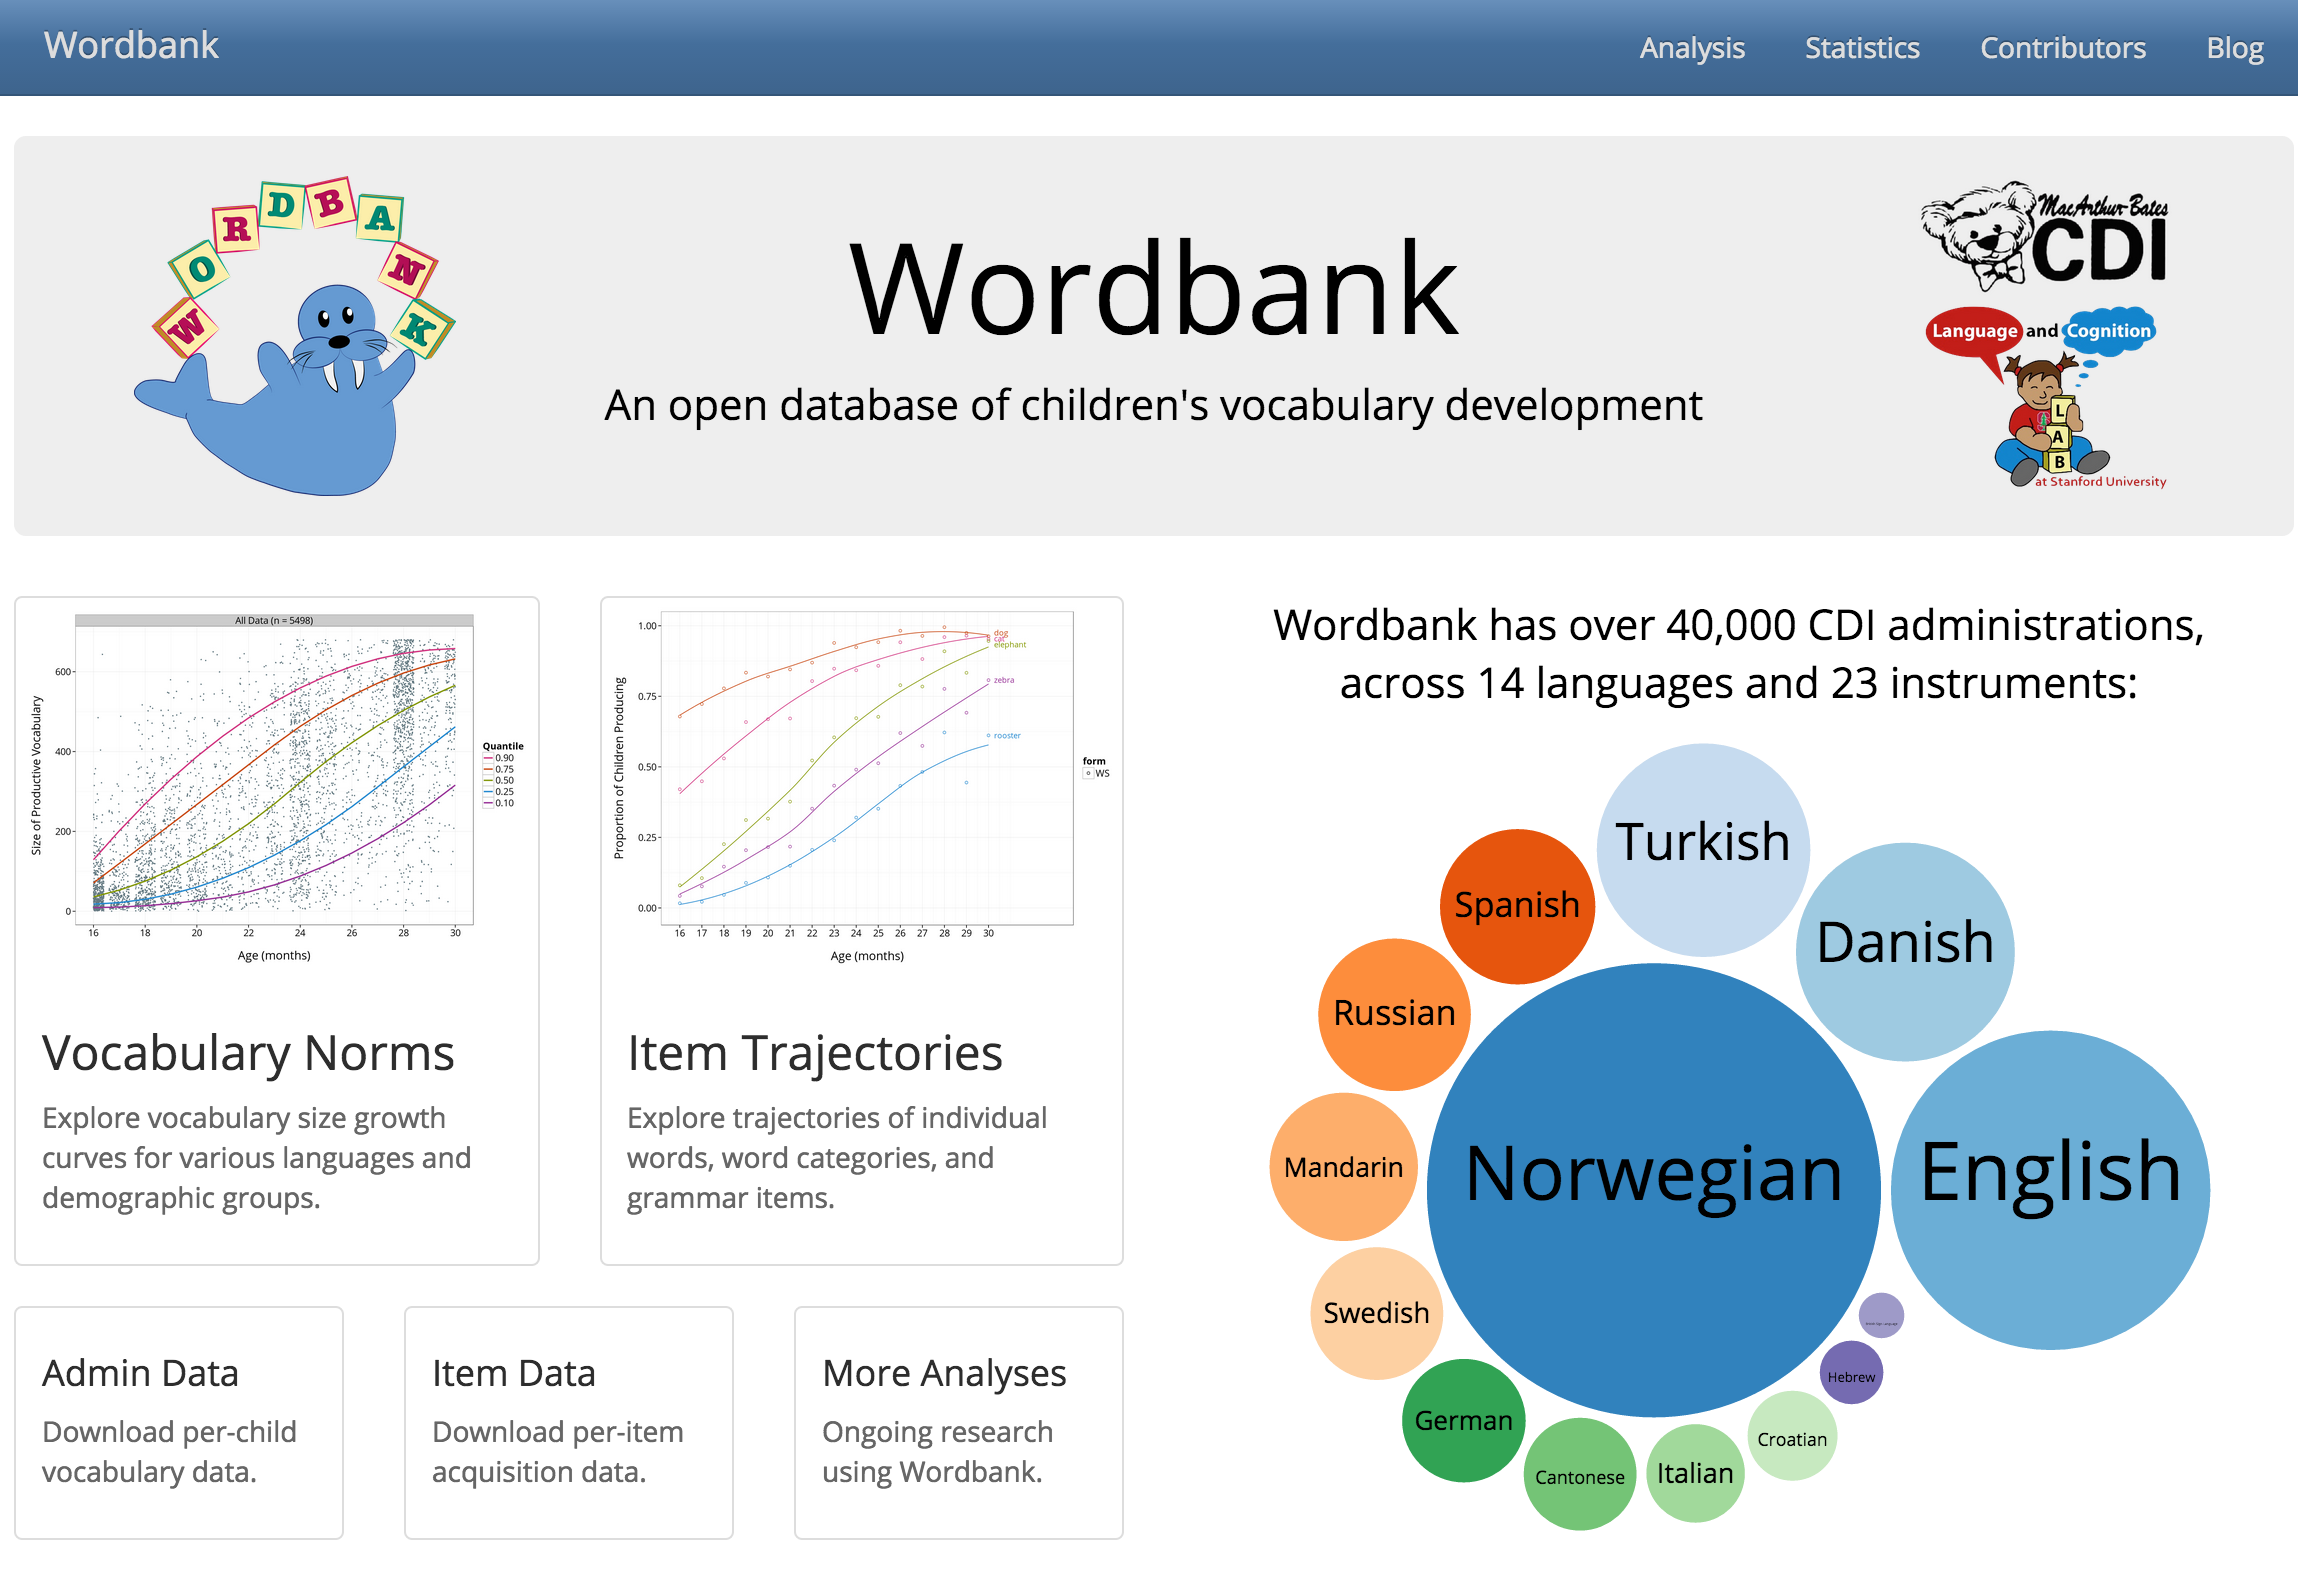
\includegraphics[width=6.4in]{figures/screenshot.png}
\caption{\label{fig:screenshot} Screenshot of the current Wordbank main page. Visitors can navigate from this page to the interactive reports, as well as to a statistics page that shows the database composition, a contributors page that shows citation information, and a blog that highlights recent updates.}
\end{figure}

Our inspiration for Wordbank comes from two successful projects for sharing data on children's language acquisition. The first is the Child Language Data Exchange System (CHILDES; \citeNP{macwhinney2000}). A database of transcripts of children's speech and speech to children, CHILDES has grown into a robust and important tool for the community, with many contributors and affiliated projects. The second is the Cross-Linguistic Lexical Norms site (CLEX; \url{www.cdi-clex.org/}; \citeNP{jorgensen2010}), which is closer in content to Wordbank, and effectively our precursor. CLEX archives normative data from a range of CDI adaptations across languages, allowing browsing of acquisition trajectories for individual items or age groups. 

Wordbank builds on CLEX, offering the same functionality but allowing flexible and interactive visualization and analysis, as well as direct database access and data download. In addition, Wordbank's goal is to extend beyond the norming data provided by the developers of individual CDIs by dynamically incorporating data from many different researchers and projects of varying sizes and scopes.  While the resulting datasets in Wordbank are likely more heterogeneous, they nevertheless have the potential to be considerably larger and more representative than the individual norming datasets.  Wordbank provides tools that enable more powerful, flexible and nuanced analyses of general trends and comparisons across sub-populations in a variety of different languages.

\subsection{Database Architecture}

\begin{figure}[t]
\centering
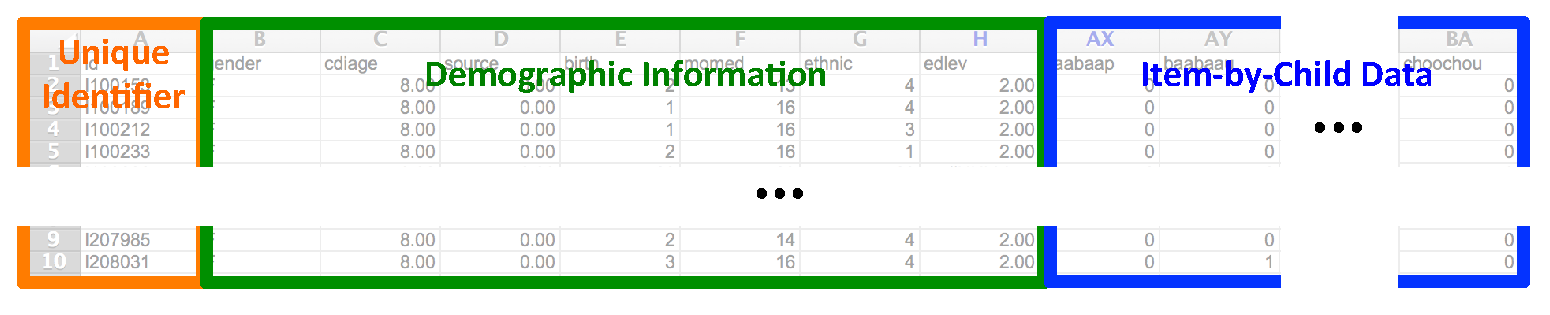
\includegraphics[width=5in]{figures/itembychild.pdf}
\caption{\label{fig:data} Example data from the CDI norming sample (Fenson et al., 2007). Each row has a unique child identifier, demographics, and word-by-word checklist data. }
\end{figure}

Why use a database to store vocabulary data? Consider the standard format of raw CDI data. Figure \ref{fig:data} shows a small slice of the original CDI norming data \cite{fenson1994,fenson2007}. Each row is a child, each column gives a variable---either a demographic variable or the result of a particular word being administered to a particular child. Although this format is useful for homogeneous administrations of a single instrument, it cannot accommodate multiple instruments, multiple languages, or datasets with different sources or kinds of demographic information. Consolidating data across different instruments is very difficult in this format, and tracking data on children with multiple longitudinal administrations of a single instrument must also be done in an ad-hoc manner. The move to a database format allows far more flexible and programmatic handling of heterogeneous data structures from different sources. 

A relational database such as Wordbank is at its heart a series of tables linked by unique identifiers. There are two primary groups of tables in Wordbank. The common tables store data that is shared between CDI instruments, including information about children, administrations (individual instances of a form being filled out for a child), and items (words and other questions on a form). The instrument tables store response data for particular CDI instruments. We currently include all items on CDI instruments, including questions about communication, gesture, morphology, and grammar, though in many of the datasets that we archive these questions have not been digitized so data on them are sparse at present. 

One strength of the Wordbank framework is that it allows the storage of subsidiary information about the words that are included in a particular instrument, so that this information can be used in future analyses. For example, information about grammatical and semantic categories or norms like concreteness and imageability could all be appended to particular words. This functionality is not yet present in wordbank, however. The difficulty of compiling this kind of information for a particular set of words is compounded by the large number of languages that the database includes. We hope that in future this functionality will allow the gradual accumulation of information about the words included in the database.

\subsubsection{Technical details}

Wordbank is constructed using free, open-source tools. The database is a standard MySQL database, managed using Python and Django. Analysis apps are constructed using the \texttt{Shiny} package for \texttt{R}, an open-source statistical programming language.  The code is hosted in a GitHub repository (\url{github.com/langcog/wordbank}) where interested users can browse, leave comments, and contribute modifications. 

All data uploaded to Wordbank are open and freely available for download, both through the site itself and through the GitHub repository. The site includes only de-identified data that cannot be linked to the parents and children who provided it. Because of these features, the Stanford Institutional Review Board has determined that the Wordbank project does not constitute human subjects research.

\subsubsection{Cross-linguistic and cross-instrument architecture}

The general philosophy of the CDI has been summarized as ``adaptation, not translation'' \cite{dale2015}. In other words, CDIs are a useful tool for many languages, but the forms differ between languages---words and even whole sections are added, dropped, and modified to ensure that the form captures the details of the particular language for which it is designed. To date, more than 60 adaptations of the original English CDI have been documented \cite{dale2011}. These forms vary widely, nowhere more so than in length and intended age range. Some forms include hundreds of items more than the original 680 words on the English Words \& Sentences form; others are so-called ``short forms'' and include only a hundred or a few hundred carefully selected words. Some are designed to capture development from the emergence of language through 3--4 years, while others are focused on very early development (like the English Words \& Gestures form, designed for 8--18 months). All of these differences make it problematic to compare scores and score distributions across forms, even using percentile ranks, since some instruments will have more or more difficult items than others. 

Wordbank is designed so that it can accommodate data from a wide variety of instruments, both within and across languages. Indeed, at the time of writing, the site includes data from more than 44,000 administrations of the CDI across 13 different languages and 23 different instruments. But because of the difficulties in comparison across instruments, our approach to cross-linguistic and cross-instrument data is to provide standardized analyses within each instrument and language, without assuming equivalence across words, instruments, or populations. Thus, our exploratory visualization tools in general do not allow comparison across languages and we urge users to interpret cross-linguistic and cross-instrument differences with caution.\footnote{The only exception to this policy currently is that we allow users to see responses across forms for individual words, in the Item Trajectories analysis. Since many of the concerns about comparing across forms center around the different items on each form, within-item analyses are likely less problematic.} Developing statistical techniques to facilitate these comparisons is a current focus of our research. 


\subsection{Interactive Analysis Tools}

The primary method for users to interact with the Wordbank is through interactive analysis tools that are hosted on the website. These tools allow for fast and flexible exploration of the dataset, the results of which can be exported in tabular and graphical formats for further analysis and presentation. 

\subsubsection{Vocabulary norms}

\begin{figure}[h!]
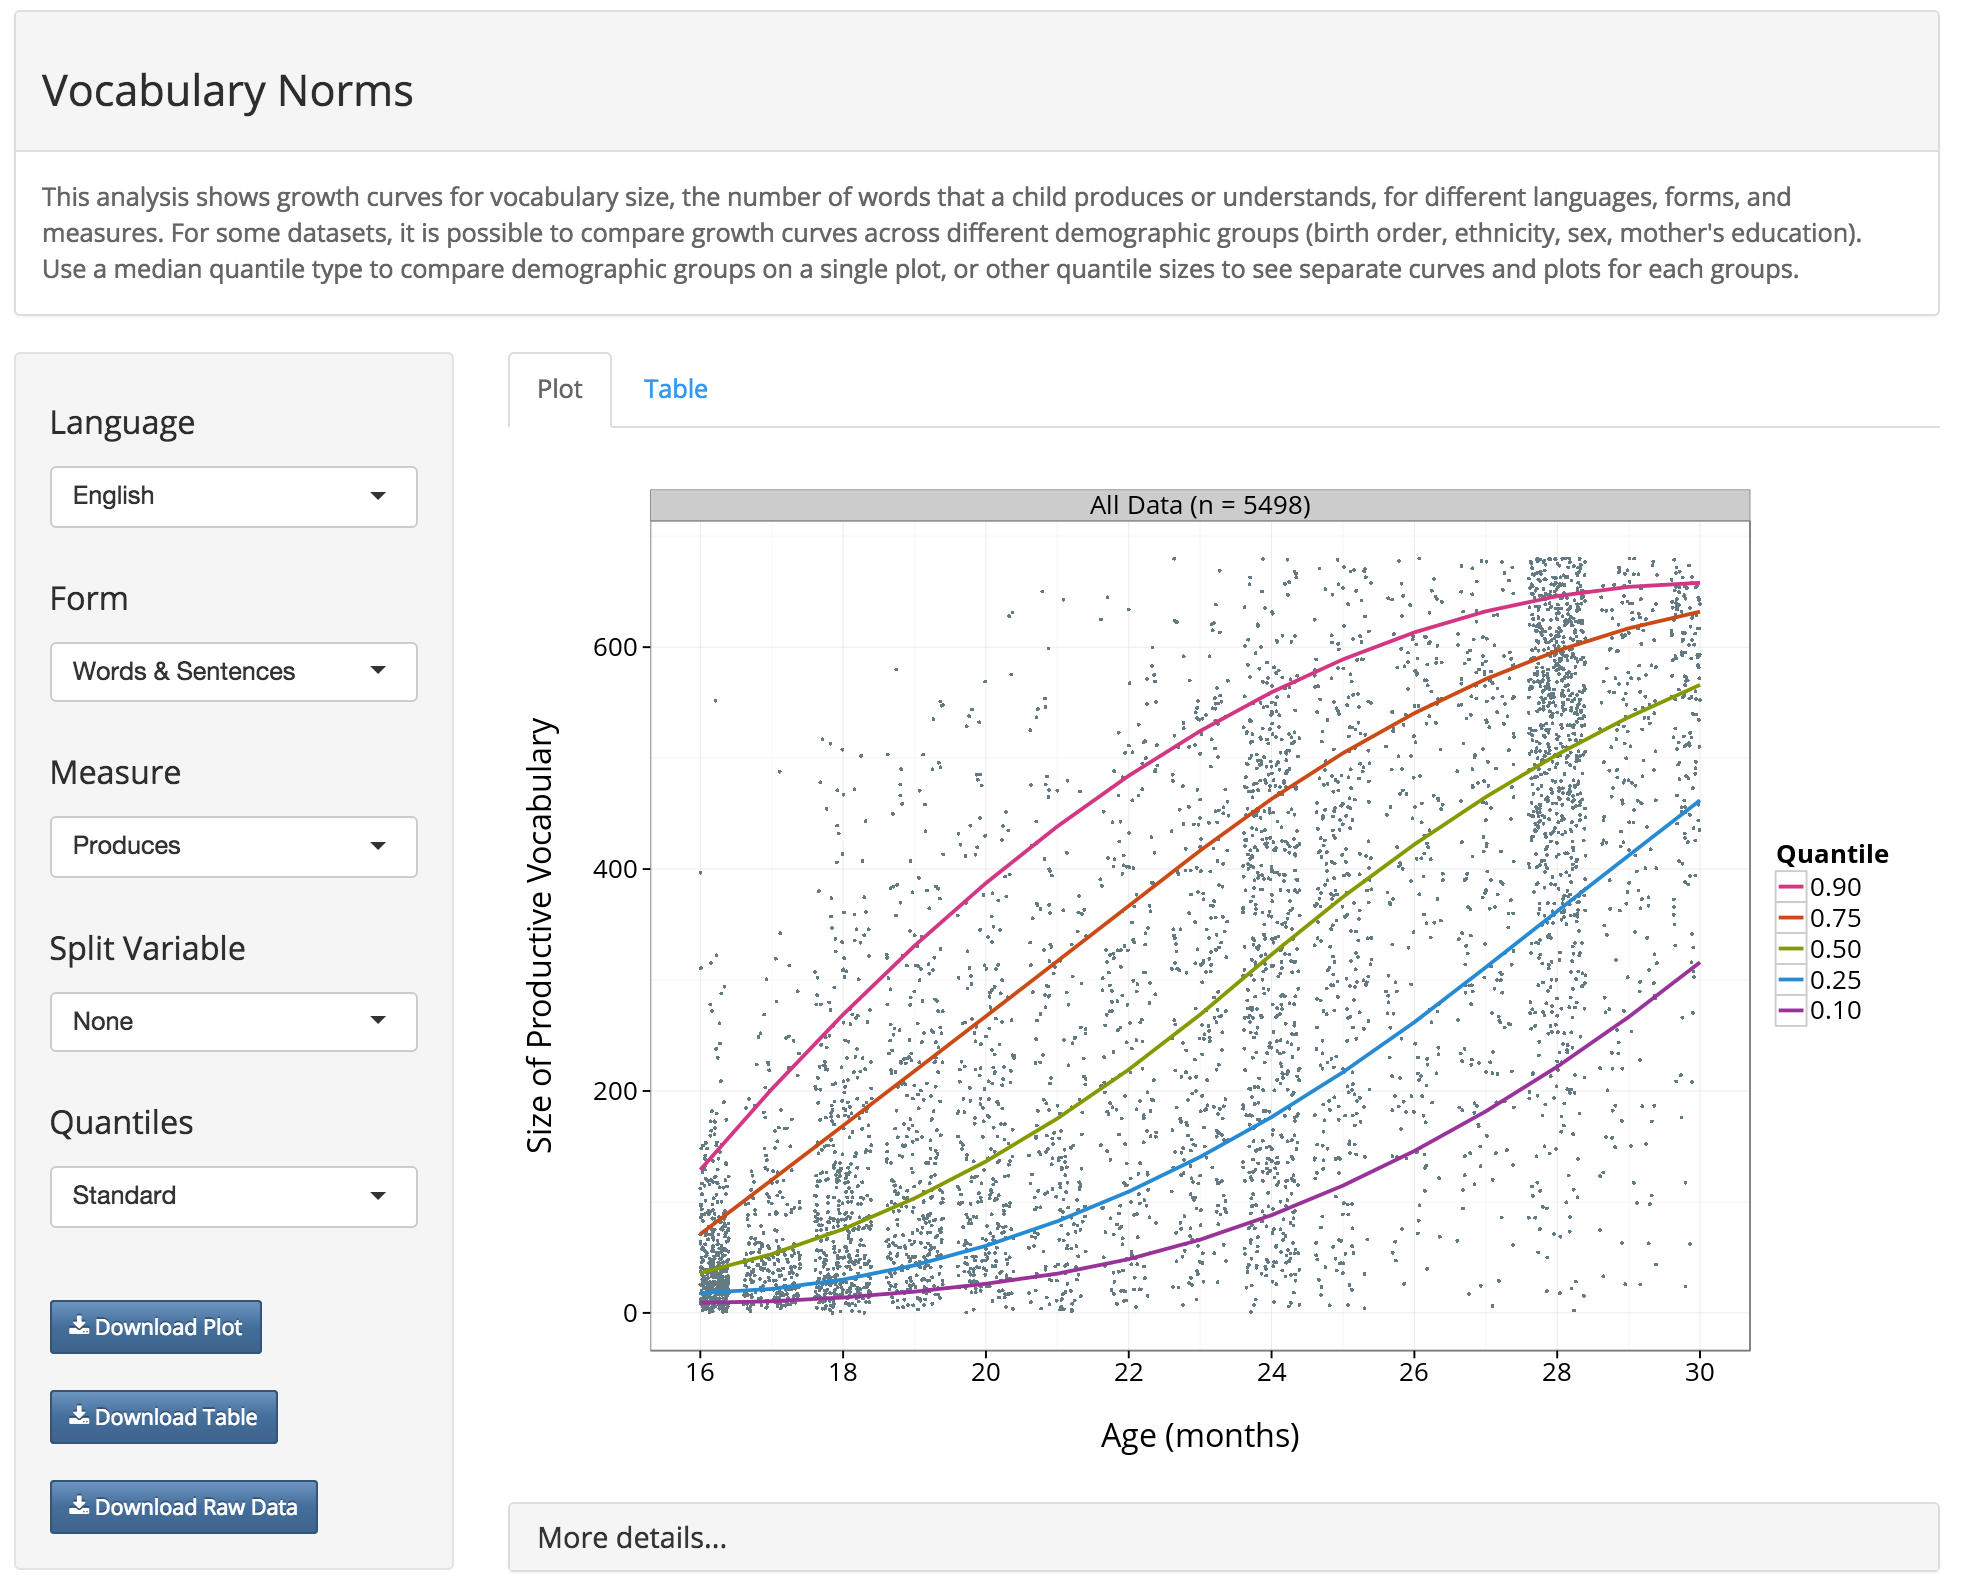
\includegraphics[width=6in]{figures/normsapp.png}
\caption{\label{fig:norms} A screenshot of the Vocabulary Norms analysis tool, showing 10th, 25th, 50th, 75th, and 90th percentiles (default) for English production scores. Dots show individual administrations, jittered slightly to avoid overplotting. Curves show polynomial spline fits (see text for more details).}
\end{figure}

One of the primary purposes of the CDI form is to provide percentile ranks for vocabulary growth across ages, both for visualizing the variability of early vocabulary growth and for examining differences in these growth patterns due to both individual differences and demographic variables. Accordingly, Wordbank provides a Vocabulary Norms analysis, pictured in Figure \ref{fig:norms}. The inset plot shows all administrations of a particular CDI instrument within the instrument's valid age range. Dots show individual children, with age binned by month and jittered to avoid overplotting. Lines on the plot indicate estimates of percentiles, fit using quantile regression with monotonic polynomial splines as the base function (using the \texttt{gcrq} function of the \texttt{quantregGrowth} package; \citeNP{muggeo2013}). An important feature of the norms app is that it can be split by any demographic field in the data, so that comparisons on variables like sex, birth order, or maternal education can be conducted across languages. 

The original and updated norming studies \cite{fenson1994,fenson2007} gathered data from a diverse (though not nationally-representative) sample and used these data to construct normative curves from which percentile ranks could be derived. In contrast to these studies, Wordbank is not explicitly designed to provide stable, clinically-relevant norms. Wordbank's sample is heterogeneous and continually growing, and its analyses are subject to revision and update. Thus, Wordbank does not currently generate percentile ranks for input data, and we do not recommend that Wordbank-generated norming values be used for research or clinical purposes in which the goal is to evaluate children's performance in reference to an established normative standard. For these types of applications, users should refer to the published norms in the appropriate language.\footnote{Users can always generate percentile ranks themselves, and this may be desirable or necessary for research purposes, but we caution against the clinical use of such ad-hoc norms.}

\subsubsection{Item trajectories}

\begin{figure}[h!]
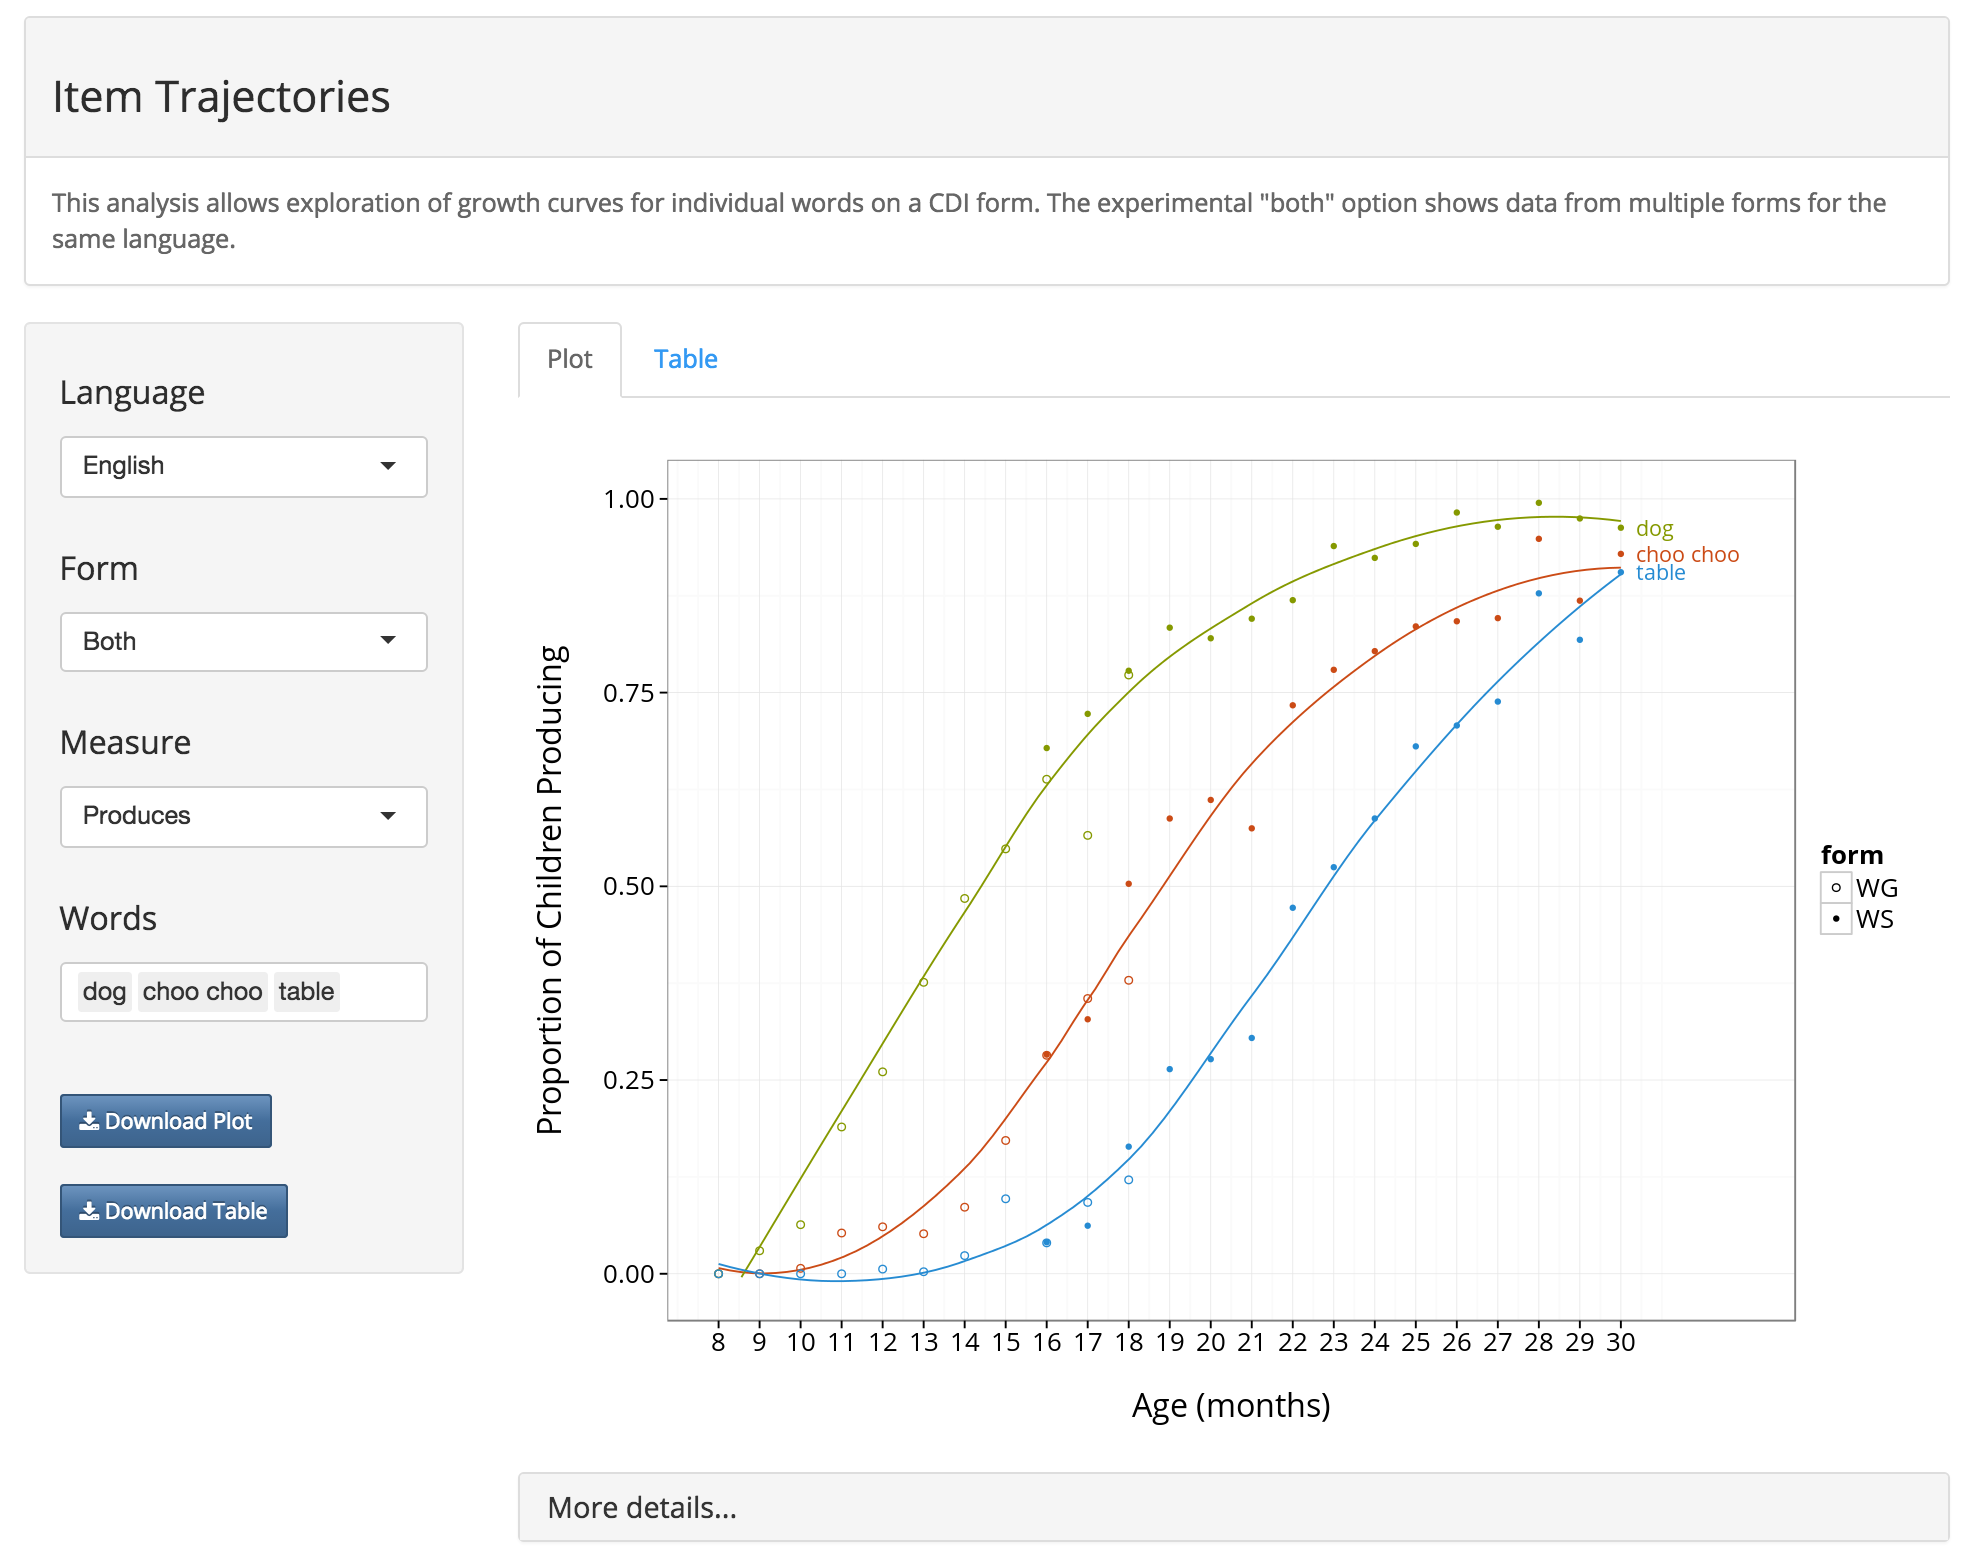
\includegraphics[width=6in]{figures/itemsapp.png}
\caption{\label{fig:items} A screenshot of the Item Trajectories analysis tool, showing a visualization of the developmental trajectory of production for three words (\emph{dog}, \emph{choo choo}, and \emph{table}) across both Words \& Gestures and Words \& Sentences forms.}
\end{figure}

A second function of the CDI form is to provide aggregate data on the proportion of children at a particular age who know a specific word \cite{dale1996,jorgensen2010}. Such analyses can be extremely helpful for the design and evaluation of materials for young children, including experimental stimuli. Accordingly, the second major interactive visualization in Wordbank is the Item Trajectories analysis tool. 

This tool allows exploration of growth curves for individual words on a CDI form. Users can select a language and instrument (and choose production or comprehension where available), and then select or input a list of words whose trajectories are plotted (Figure \ref{fig:items}). The ``both'' measure option shows data from multiple forms for the same language, with different markers for each item. In general, our exploration suggests that there are only small differences across different instruments for the same item and age. Lines on the plot show a local polynomial regression smoothing line (\texttt{loess} in \texttt{R}). 

\subsubsection{Other features: Static reports and tabular data download}

In addition to the interactive analysis tools described above, Wordbank also includes a number of non-interactive but continuously updated reports on features like vocabulary composition across languages, links between grammar and the lexicon \cite{braginsky2015}, and gender differences in vocabulary growth (see below). On the Analysis page (\url{wordbank.stanford.edu/reports}), we provide a gallery of both interactive and non-interactive analyses. 

Wordbank also allows raw tabular data to be browsed and downloaded for subsequent analysis in all popular statistical packages. Using the same basic interface as the Vocabulary Norms and Item Trajectory tools, users can browse raw data aggregated across children (similar to the Vocabulary Norms tool), across items (similar to the Items Trajectory tool), or even view the raw subject-by-item data. All data in these ``standard'' reports can be downloaded in CSV format. 

\subsection{Extensibility}

Extensibility is one of the major strengths of Wordbank. Although programming knowledge is not necessary for interacting with Wordbank, interested researchers with programming skills can contribute to the development effort by adding new analyses. Each Wordbank analysis app is constructed as a standalone script or set of scripts in the \texttt{R} language. Constructing an interactive analysis requires specifying a visualization and some interactive functionality using \texttt{Shiny}. Non-interactive analyses can be constructed as \texttt{R Markdown} documents that execute scripts using the Wordbank database. Both of these have the virtue of rerunning on the newest version of the database whenever they are opened, so they do not go out of date as new data are added. 

In addition, we encourage contributions of individual datasets. Wordbank currently imports data from Excel and CSV formats via automated import scripts. Individuals or labs interested in contributing should consult with the authors for advice about data formatting and upload. 

\section{\texttt{wordbankr}: an \texttt{R} package for accessing Wordbank}

Although the analysis tools described above suffice for many needs, researchers interested in detailed quantitative or cross-linguistic analyses may wish to connect directly to the Wordbank database and manipulate the data directly. Making use of the \texttt{R} programming language \cite{team2014}, we provide the \texttt{wordbankr} package to help researchers accomplish this task. R is an open-source, extensible statistical computing environment that is rapidly growing in popularity across fields and in increasing use in child language research \cite<e.g.>{song2015,norrman2015}. The \texttt{wordbankr} package abstracts away the details of connecting to the database. Users can take advantage of the SQL tools developed in the popular \texttt{dplyr} package \cite{wickham2014}, which make manipulating large datasets quick and easy. We describe the commands that the package provides and then give a worked example of using the package for a simple analysis.

\subsection{Package details}

The \texttt{wordbankr} package is easily installed via CRAN, the comprehensive R archive network. To install, simply type: \texttt{install.packages(``wordbankr'')}. After installation, the first step in using \texttt{wordbankr} is to connect to the database using the \texttt{connect\char`_to\char`_wordbank} command. Users can connect in \texttt{remote} mode, which loads data from the Wordbank server, or in \texttt{local} mode if they have a copy of the database set up on their local machine. This connection can then be used to load any of the common tables by name with \texttt{get\char`_common\char`_table} and any of the instrument tables by language and form with \texttt{get\char`_instrument\char`_table}. The package also provides functions that make loading components of the data easier by joining together relevant tables to give different views of the data: by-administration (\texttt{get\char`_administration\char`_data}) with demographics and vocabulary sizes; by-item (\texttt{get\char`_item\char`_data}) with item types, categories and other information; or administration-by-item (\texttt{get\char`_instrument\char`_data}) with raw response values. For more detailed documentation, see the package repository (\url{http://github.com/langcog/wordbankr}).

\subsection{A worked example: Gender differences across languages}

We demonstrate the analytic potential of direct manipulation of the Wordbank database using \texttt{wordbankR}. Our example is an analysis examining gender differences.\footnote{The distinction between sex (biological characteristic) and gender (social characteristic) is complex, and not well-understood in early childhood. We defer discussion of this issue, but since the CDI is a parent-report form we do not have access to sex information directly. Instead, we describe parents' reports as reflecting gender rather than sex.} Gender differences in productive language are commonly found in individual studies (e.g., \citeNP{fenson1994,huttenlocher1991}; see \citeNP{wallentin2009} for review), and one large-scale previous study found differences in productive vocabulary in 10 languages \cite{eriksson2012}. In the following analysis, we show how this general analysis can quickly be replicated using Wordbank.

To perform the analysis, we first begin by using \texttt{wordbankr} to load the data from Wordbank and connect to the tables we need:

\begin{lstlisting}
admins <- get_administration_data()
items <- get_item_data()
\end{lstlisting}

\noindent We next use a series of \texttt{dplyr} calls to compute the number of words in each language,  select the appropriate subset of the data, and calculate the proportion of words produced for this data subset:

\begin{lstlisting}
num_words <- items %>%
  filter(form == "WS", type == "word") %>%
  group_by(language) %>%
  summarise(n = n())

vocab_admins <- admins %>%
  select(data_id, language, form, age, sex, production)

vocab_data <- vocab_admins %>%
  group_by(language, sex, age) %>%
  left_join(num_words) %>%
  mutate(production = as.numeric(production) / n) %>%
  summarise(median = median(production))
\end{lstlisting}

\noindent We then plot the \texttt{vocab\char`_data} data frame using the \texttt{ggplot2} library \cite{wickham2009}. Full code for the analysis as a whole (including the plot) is given in the Using Wordbank tutorial, available on at \url{wordbank.stanford.edu/tutorial}.

\begin{figure}[ht!]
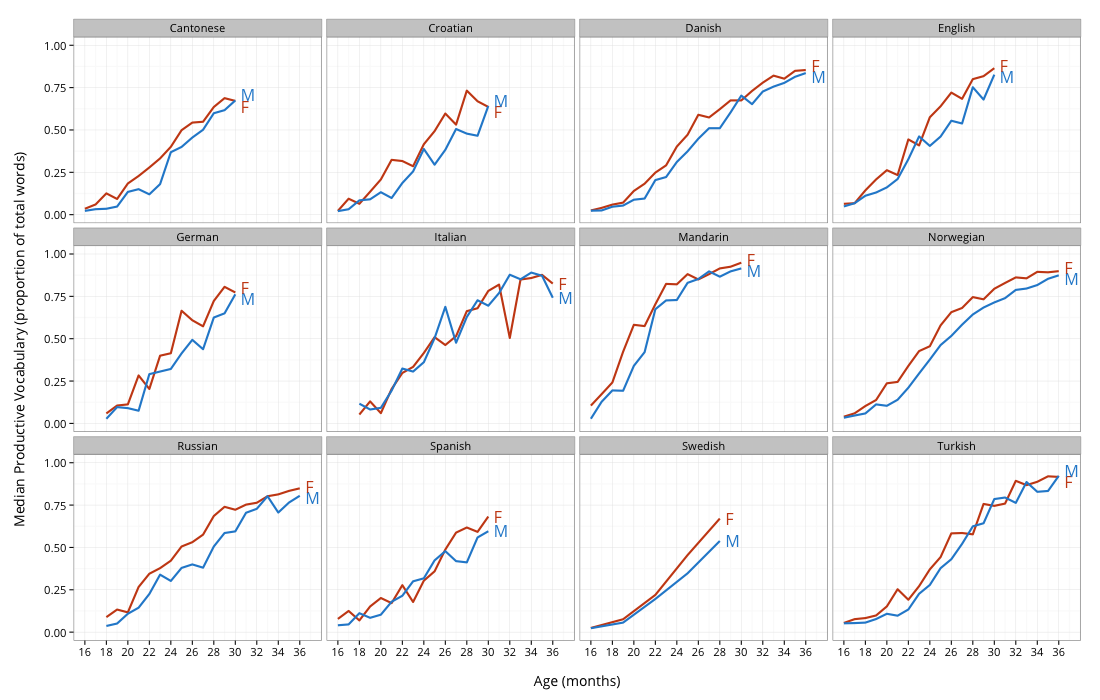
\includegraphics[width=6in]{figures/gender.png}
\caption{\label{fig:gender} Median productive vocabulary as a proportion of total words on an instrument, plotted by age in months. Red and blue lines show females and males, respectively.}
\end{figure}

The results of this analysis are shown in Figure \ref{fig:gender}. As expected, we replicate the gender differences found in previous work: Female showed a small but highly reliable advantage in early production. This effect is highly consistent and clearly visible in 11 out of 12 languages, with Italian being the only exception. While the Wordbank data do not allow us to speculate about the origins of this difference, they certainly allow us to formulate hypotheses with substantially more clarity than previous analyses. Such visualizations also highlight differences in the size and composition of the database.

\section{Conclusions}

In this paper, we presented Wordbank, an open repository for parent-report vocabulary data using the MacArthur-Bates CDI. The interactive analysis tools available on the Wordbank site allow interested researchers to explore a wide variety of phenomena in vocabulary development quickly and easily, exporting data and downloading presentation-quality graphics that document their analysis. In addition, users can contribute new analyses and data to the site and connect to it directly using an \texttt{R} package for data loading. These functions all enable greater sharing and reuse of existing data on children's vocabulary. We hope that the resulting tools will enable new discoveries in the future.

\bibliographystyle{apacite}
\bibliography{wordbank}

\end{document}
